% konsolidierung_1983_1998.tex
\chapter{Konsolidierung und neoliberale Wende (1983–1998)}
\label{chap:konsolidierung}

\section*{Einleitung}
Die Jahre 1983 bis 1998 umfassen zwei politische Ären: Die konservative Regierung Helmut Kohls (1983–1998) und den Beginn der rot-grünen Koalition
(ab 1998). Diese Periode war geprägt von wirtschaftlicher Konsolidierung, strukturellen Reformen und der Vollendung der deutschen
Einheit – gleichzeitig aber auch von wachsender sozialer Spaltung und der Durchsetzung neoliberaler Politikparadigmen.

\section{Kontext: Der neoliberale Paradigmenwechsel}

\begin{itemize}
    \item \textbf{Wende 1982/83}: \enquote{Geistig-moralische Wende} unter Helmut Kohl
    \item \textbf{Deutsche Einheit 1990}: Wirtschaftliche und soziale Herausforderungen
    \item \textbf{Globalisierung}: Liberalisierung der Finanzmärkte, Standortwettbewerb
    \item \textbf{EU-Integration}: Maastricht-Vertrag (1992), Einführung des Euro beschlossen
\end{itemize}

Diese Ära markiert den Übergang vom keynesianischen Wohlfahrtsstaat zum neoliberalen Wettbewerbsstaat.

\begin{table}[ht]
    \centering
    \caption{Makroökonomische Entwicklung 1983–1998}
    \label{tab:makro_konsolidierung}
    \begin{tabular}{lcccc}
        \toprule
        \textbf{Periode} & \textbf{BIP-Wachstum} & \textbf{Arbeitslosenquote} & \textbf{Staatsverschuldung} & \textbf{Lohnstückkosten} \\
        & \textbf{(\% p.a.)} & \textbf{(\%)} & \textbf{(\% BIP)} & \textbf{(1991=100)} \\
        \midrule
        1983–1989 & 2.4 & 8.6 & 41.9 & 98.2 \\
        1990–1994 & 3.1 & 8.5 & 47.3 & 112.4 \\
        1995–1998 & 1.7 & 10.3 & 60.1 & 105.8 \\
        \midrule
        \textbf{Gesamt} & \textbf{2.4} & \textbf{9.1} & \textbf{49.8} & \textbf{105.5} \\
        \bottomrule
    \end{tabular}
\end{table}

\begin{flushleft}
\footnotesize{\textit{Quelle: Statistisches Bundesamt, Sachverständigenrat. Arbeitslosigkeit blieb strukturell hoch, Staatsverschuldung stieg durch die Einheit.}}
\end{flushleft}

\section{GWI-D Entwicklung: Stabilisierung auf niedrigem Niveau}

\begin{table}[ht]
    \centering
    \caption{GWI-D Komponenten 1983–1998}
    \label{tab:gwi_konsolidierung}
    \begin{tabular}{lccccc}
        \toprule
        \textbf{Jahr} & \textbf{W (\(W\))} & \textbf{G (\(G\))} & \textbf{Z (\(Z\))} & \textbf{S (\(S\))} & \textbf{GWI-D} \\
        \midrule
        1983 & 75.8 & 69.5 & 67.1 & 74.8 & 73.8 \\
        1985 & 78.3 & 70.2 & 68.9 & 75.3 & 75.2 \\
        1987 & 80.1 & 71.0 & 70.5 & 75.9 & 76.4 \\
        1989 & 82.4 & 71.8 & 72.1 & 76.5 & 78.2 \\
        1991 & 79.6 & 69.2 & 68.8 & 74.1 & 74.9 \\
        1993 & 76.8 & 67.9 & 66.4 & 72.8 & 72.5 \\
        1995 & 78.2 & 68.5 & 67.9 & 73.5 & 73.8 \\
        1997 & 79.7 & 69.8 & 69.4 & 74.2 & 75.1 \\
        1998 & 80.5 & 70.1 & 70.2 & 74.8 & 75.9 \\
        \midrule
        \textbf{Durchschnitt} & \textbf{79.0} & \textbf{69.8} & \textbf{69.0} & \textbf{74.7} & \textbf{75.1} \\
        \textbf{Änderung} & \textbf{+4.7} & \textbf{+0.6} & \textbf{+3.1} & \textbf{0.0} & \textbf{+2.1} \\
        \bottomrule
    \end{tabular}
\end{table}

\begin{flushleft}
\footnotesize{\textit{Anmerkung: Geringe Veränderungen über 16 Jahre – Stagnation auf mittlerem Niveau.}}
\end{flushleft}

\subsection{Wirtschaftliche Erholung mit Grenzen (\(W\))}

Die Wirtschaftskomponente stieg von 75,8 (1983) auf 80,5 (1998) – eine leichte Erholung um 4,7 Punkte nach der Stagflation.

\textbf{Positive Entwicklungen}:
\begin{itemize}
    \item \textbf{Exportboom}: Deutsche Exporte verdoppelten sich (1983: 340 Mrd DM → 1998: 680 Mrd DM)
    \item \textbf{Produktivitätssteigerung}: Industrieroboter, Computerisierung, Lean Production
    \item \textbf{Dienstleistungssektor}: Anteil stieg von 58\% auf 68\% der Beschäftigung
\end{itemize}

\textbf{Strukturelle Probleme}:
\begin{itemize}
    \item \textbf{Deutschland als „kranker Mann Europas"}: Hohe Lohnkosten, geringe Flexibilität
    \item \textbf{Investitionsschwäche}: Reale Investitionsquote sank von 23\% auf 20\%
    \item \textbf{Einheitslasten}: Geschätzte Kosten von 1,5 Billionen DM für die deutsche Einheit
\end{itemize}

\subsection{Gerechtigkeitsstagnation (\(G\))}

Die Gerechtigkeitskomponente blieb mit nur +0,6 Punkten nahezu unverändert – das \textbf{zweitniedrigste Ergebnis} aller Komponenten.

\begin{figure}[ht]
    \centering
    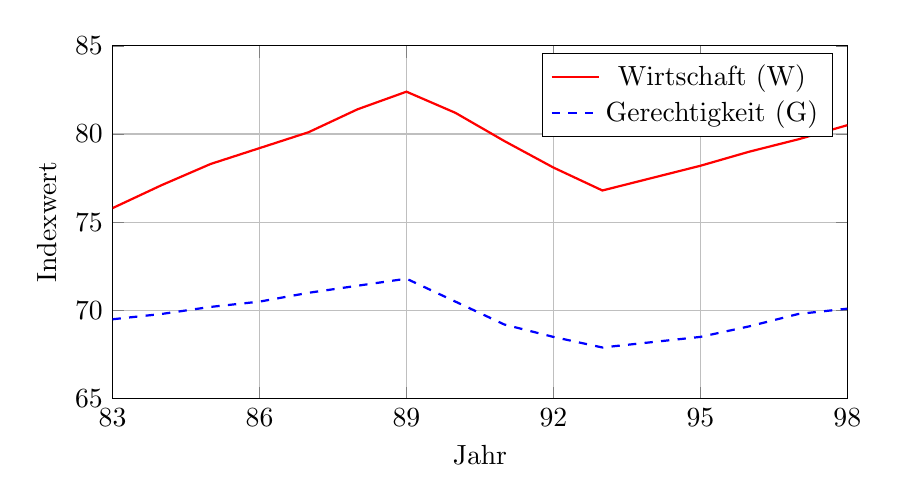
\begin{tikzpicture}
        \begin{axis}[
            width=0.9\textwidth,
            height=0.5\textwidth,
            xlabel={Jahr},
            ylabel={Indexwert},
            xmin=1983, xmax=1998,
            ymin=65, ymax=85,
            grid=both,
            legend style={at={(0.98,0.98)}, anchor=north east},
            xtick={1983,1986,1989,1992,1995,1998},
            xticklabels={83,86,89,92,95,98},
            ]
            \addplot[color=red, thick] coordinates {
                (1983,75.8) (1984,77.1) (1985,78.3) (1986,79.2)
                (1987,80.1) (1988,81.4) (1989,82.4) (1990,81.2)
                (1991,79.6) (1992,78.1) (1993,76.8) (1994,77.5)
                (1995,78.2) (1996,79.0) (1997,79.7) (1998,80.5)
            };
            \addplot[color=blue, thick, dashed] coordinates {
                (1983,69.5) (1984,69.8) (1985,70.2) (1986,70.5)
                (1987,71.0) (1988,71.4) (1989,71.8) (1990,70.5)
                (1991,69.2) (1992,68.5) (1993,67.9) (1994,68.2)
                (1995,68.5) (1996,69.1) (1997,69.8) (1998,70.1)
            };
            \legend{Wirtschaft (W), Gerechtigkeit (G)}
        \end{axis}
    \end{tikzpicture}
    \caption{Entwicklung 1983–1998: Wirtschaft erholt sich, Gerechtigkeit stagniert}
    \label{fig:entwicklung_konsolidierung}
\end{figure}

\begin{flushleft}
\footnotesize{\textit{Anmerkung: Die deutsche Einheit 1990 führte zu einem temporären Einbruch beider Komponenten.}}
\end{flushleft}

\textbf{Ursachen der Gerechtigkeitsstagnation}:

\begin{itemize}
    \item \textbf{Arbeitsmarktdualismus}: Wachsende Kluft zwischen Kernbelegschaften und Randbelegschaften
    \item \textbf{Steuerpolitik}: Senkung der Spitzensteuersätze von 56\% auf 53\% (1990) bzw. 47\% (1998)
    \item \textbf{Sozialabbau}: Leistungskürzungen bei Arbeitslosen- und Krankenversicherung
    \item \textbf{Regionale Spaltung}: Ostdeutschland: 18\% Arbeitslosigkeit vs. West: 8\%
\end{itemize}

\subsection{Zukunft (\(Z\)) und Zusammenhalt (\(S\))}

\begin{itemize}
    \item \textbf{Zukunft (\(Z\))}: +3,1 Punkte – Umweltbewegung (Tschernobyl 1986), Bildungsreformen, aber auch Forschungsdefizite
    \item \textbf{Zusammenhalt (\(S\))}: 0,0 Punkte Veränderung – Einheit als Belastung, wachsende Fremdenfeindlichkeit (1992: Rostock, Mölln)
\end{itemize}

\section{Soziale Entwicklungen: Die Spaltung vertieft sich}

\begin{table}[ht]
    \centering
    \caption{Soziale Indikatoren 1983–1998}
    \label{tab:sozial_konsolidierung}
    \begin{tabular}{lccc}
        \toprule
        \textbf{Indikator} & \textbf{1983} & \textbf{1998} & \textbf{Veränderung} \\
        \midrule
        Arbeitslosenquote (\%) & 8.6 & 10.3 & +1.7 PP \\
        Langzeitarbeitslose (Mio.) & 0.8 & 1.6 & +100\% \\
        Niedriglohnsektor (\% Besch.) & 12.4 & 18.7 & +6.3 PP \\
        Gini-Koeffizient (Einkommen) & 0.291 & 0.317 & +0.026 \\
        Armutsquote (\%) & 9.8 & 12.1 & +2.3 PP \\
        Managergehälter (x Facharbeiter) & 12 & 28 & +133\% \\
        \bottomrule
    \end{tabular}
\end{table}

\begin{flushleft}
\footnotesize{\textit{Quelle: SOEP, IAB, Statistisches Bundesamt. Deutliche Zunahme sozialer Ungleichheit.}}
\end{flushleft}

\textbf{Kritische Trends}:

\begin{itemize}
    \item \textbf{Massenarbeitslosigkeit als Dauerzustand}: Über 4 Millionen Arbeitslose 1998
    \item \textbf{Prekarisierung}: Leiharbeit stieg um 180\%, befristete Verträge um 95\%
    \item \textbf{Einkommenspolarisierung}: Reale Nettolöhne stagnierten, Kapitaleinkommen stiegen um 45\%
    \item \textbf{Regionale Disparitäten}: Ost-West-Gefälle, aber auch Nord-Süd-Gefälle im Westen
\end{itemize}

\section{Die deutsche Einheit als Belastungsprobe}

Die Wiedervereinigung 1990 war ein \textbf{historischer Glücksfall mit hohen sozialen Kosten}:

\begin{table}[ht]
    \centering
    \caption{GWI-D Entwicklung um die deutsche Einheit}
    \label{tab:einheit_gwi}
    \begin{tabular}{lccccc}
        \toprule
        \textbf{Jahr} & \textbf{W (\(W\))} & \textbf{G (\(G\))} & \textbf{Z (\(Z\))} & \textbf{S (\(S\))} & \textbf{GWI-D} \\
        \midrule
        1989 (vor Einheit) & 82.4 & 71.8 & 72.1 & 76.5 & 78.2 \\
        1991 (nach Einheit) & 79.6 & 69.2 & 68.8 & 74.1 & 74.9 \\
        \textbf{Differenz} & \textbf{-2.8} & \textbf{-2.6} & \textbf{-3.3} & \textbf{-2.4} & \textbf{-3.3} \\
        \bottomrule
    \end{tabular}
\end{table}

\begin{flushleft}
\footnotesize{\textit{Anmerkung: Kurzfristiger Einbruch aller Komponenten durch die Einheitskosten.}}
\end{flushleft}

\textbf{Soziale Folgen der Einheit}:
\begin{itemize}
    \item \textbf{Deindustrialisierung Ost}: Verlust von 2,5 Millionen Arbeitsplätzen (1989–1993)
    \item \textbf{Aufbau Ost}: 1,5 Billionen DM Transferleistungen (1990–1998)
    \item \textbf{Mentalitätsunterschiede}: \enquote{Besserwessis} vs. \enquote{Jammerossis}
    \item \textbf{Rechtsextremismus}: Anschläge in Hoyerswerda (1991), Rostock (1992)
\end{itemize}

\section{Korrelationen: Wirtschaft dominiert, Soziales marginalisiert}

\begin{table}[ht]
    \centering
    \caption{Korrelationen zwischen GWI-D Komponenten 1983–1998}
    \label{tab:korrelation_konsolidierung}
    \begin{tabular}{lcccc}
        \toprule
        & \textbf{W (\(W\))} & \textbf{G (\(G\))} & \textbf{Z (\(Z\))} & \textbf{S (\(S\))} \\
        \midrule
        \textbf{W (\(W\))} & 1.00 & 0.32 & 0.78 & 0.65 \\
        \textbf{G (\(G\))} & 0.32 & 1.00 & 0.41 & 0.52 \\
        \textbf{Z (\(Z\))} & 0.78 & 0.41 & 1.00 & 0.68 \\
        \textbf{S (\(S\))} & 0.65 & 0.52 & 0.68 & 1.00 \\
        \bottomrule
    \end{tabular}
\end{table}

\begin{flushleft}
\footnotesize{\textit{Anmerkung: Wirtschaft (W) und Gerechtigkeit (G) korrelieren nur schwach (r=0,32).}}
\end{flushleft}

Die Korrelationsanalyse zeigt:
\begin{itemize}
    \item \textbf{Schwache Wirtschaft-Gerechtigkeit-Kopplung}: Wachstum kommt nicht bei allen an
    \item \textbf{Wirtschaft dominiert Zukunft}: Investitionen in Zukunft sind wirtschaftsabhängig
    \item \textbf{Relative Stärke des Zusammenhalts}: S korreliert besser mit G (0,52) als W mit G (0,32)
\end{itemize}

\section{Politische Reformen und ihre Wirkung}

\begin{table}[ht]
    \centering
    \caption{Wichtige Reformen und GWI-D-Wirkung}
    \label{tab:reformen_konsolidierung}
    \begin{tabular}{llcc}
        \toprule
        \textbf{Jahr} & \textbf{Reform} & \textbf{$\Delta$ GWI-D} & \textbf{Hauptwirkung} \\
        \midrule
        1984 & Haushaltskonsolidierung & -0,8 & Soziale Kürzungen \\
        1986 & Steuerreform & +0,4 & Wirtschaftliche Stimulierung \\
        1989 & Rentenreform & -0,6 & Leistungskürzungen \\
        1992 & Maastricht-Vertrag & +0,3 & Europäische Integration \\
        1994 & Solidarpakt & +0,5 & Ost-West-Ausgleich \\
        1996 & Sparpaket (\enquote{Kohl-Paket}) & -1,2 & Sozialer Rückschritt \\
        1998 & Rot-Grün-Wahl & +0,7 & Politische Hoffnung \\
        \bottomrule
    \end{tabular}
\end{table}

\begin{flushleft}
\footnotesize{\textit{Anmerkung: Sparpolitik wirkte negativ auf GWI-D, europäische Integration positiv.}}
\end{flushleft}

\textbf{Politische Paradigmen}:
\begin{itemize}
    \item \textbf{Konservative Ära (Kohl)}: Angebotspolitik, Schuldenabbau, soziale Kürzungen
    \item \textbf{Rot-Grüne Wende (ab 1998)}: Ökologische Modernisierung, aber auch \enquote{Agenda 2010} angelegt
\end{itemize}

\section{Die neoliberale Wende: Gewinner und Verlierer}

\begin{figure}[ht]
    \centering
    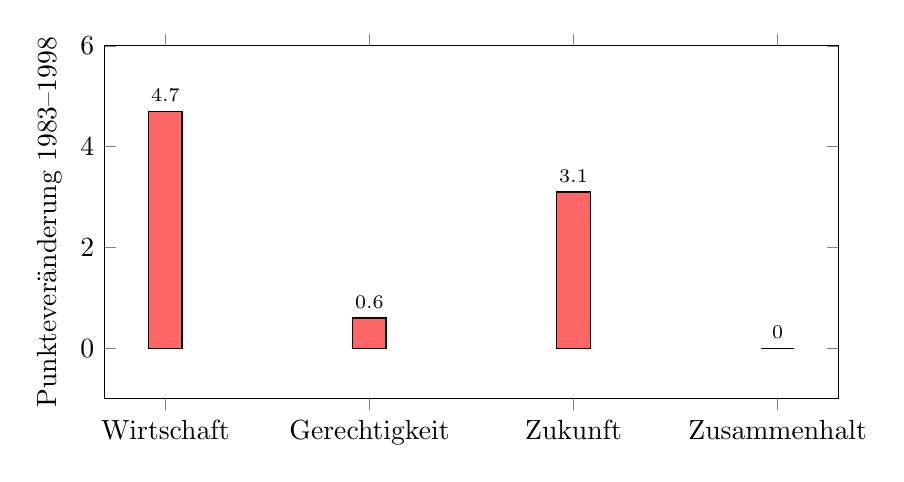
\begin{tikzpicture}
        \begin{axis}[
            width=0.9\textwidth,
            height=0.5\textwidth,
            ybar,
            bar width=12pt,
            symbolic x coords={Wirtschaft, Gerechtigkeit, Zukunft, Zusammenhalt},
            xtick=data,
            ylabel={Punkteveränderung 1983–1998},
            ymin=-1, ymax=6,
            nodes near coords,
            nodes near coords align={vertical},
            every node near coord/.append style={font=\scriptsize},
            ]
            \addplot[fill=red!60] coordinates {
                (Wirtschaft, 4.7)
                (Gerechtigkeit, 0.6)
                (Zukunft, 3.1)
                (Zusammenhalt, 0.0)
            };
        \end{axis}
    \end{tikzpicture}
    \caption{GWI-D Komponenten: Wirtschaft profitiert, Soziales stagniert}
    \label{fig:gewinner_konsolidierung}
\end{figure}

\begin{flushleft}
\footnotesize{\textit{Anmerkung: Deutliche Asymmetrie zugunsten der Wirtschaftskomponente.}}
\end{flushleft}

\subsection{Gewinner der neoliberalen Wende}

\begin{itemize}
    \item \textbf{Exportindustrie}: Automobil-, Maschinenbau-, Chemieindustrie
    \item \textbf{Finanzsektor}: Banken, Versicherungen, Investmentgesellschaften
    \item \textbf{Hochqualifizierte}: Ingenieure, IT-Spezialisten, Manager
    \item \textbf{Kapitalbesitzer}: Reale Vermögensrenditen von 4–6\% p.a.
\end{itemize}

\subsection{Verlierer der neoliberalen Wende}

\begin{itemize}
    \item \textbf{Geringqualifizierte}: Arbeitslose, Langzeitarbeitslose
    \item \textbf{Ostdeutsche}: 18\% Arbeitslosigkeit, Abwanderung von 1,2 Millionen Menschen
    \item \textbf{Frauen}: Teilzeitfalle, Lohnungleichheit von 23\%
    \item \textbf{Junge Generation}: Ausbildungskrise, prekäre Beschäftigung
\end{itemize}

\section{Resümee: Die Kosten der Konsolidierung}

Die Ära 1983–1998 war geprägt von \textbf{wirtschaftlicher Stabilisierung bei sozialer Stagnation}:

\subsection{1. Der Preis der deutschen Einheit}

\begin{itemize}
    \item \textbf{Wirtschaftlich}: Hohe Transferleistungen, aber auch Wachstumsimpulse
    \item \textbf{Sozial}: Tiefe Spaltung zwischen Ost und West, mentale Gräben
    \item \textbf{Politisch}: Erfolgreiche Integration, aber soziale Unzufriedenheit
\end{itemize}

\subsection{2. Der neoliberale Paradigmenwechsel}

\begin{itemize}
    \item \textbf{Marktliberalisierung}: Deregulierung, Privatisierung, Flexibilisierung
    \item \textbf{Staatsrückzug}: Abbau von Regulationen, Sozialkürzungen
    \item \textbf{Globalisierung}: Standortwettbewerb, Lohnzurückhaltung
\end{itemize}

\subsection{3. Die wachsende soziale Spaltung}

\begin{itemize}
    \item \textbf{Einkommensungleichheit}: Gini-Koeffizient stieg kontinuierlich
    \item \textbf{Arbeitsmarktdualismus}: Kern- vs. Randbelegschaften
    \item \textbf{Regionale Disparitäten}: Ost-West, Nord-Süd, Stadt-Land
\end{itemize}

\textbf{Fazit}: Die Jahre 1983–1998 waren eine \textbf{Ära der Widersprüche}:

\begin{itemize}
    \item \textbf{Wirtschaftlich}: Stabilisierung, Exportrekorde, aber Investitionsschwäche
    \item \textbf{Sozial}: Stagnation der Gerechtigkeit, wachsende Ungleichheit
    \item \textbf{Politisch}: Erfolgreiche Einheit, aber soziale Kosten
    \item \textbf{Gesellschaftlich}: Wohlstand für viele, aber Abstieg für einige
\end{itemize}

Die GWI-D-Analyse zeigt deutlich: Die \textbf{neoliberale Wende verbesserte die Wirtschaftskomponente (+4,7), ließ aber die Gerechtigkeitskomponente nahezu unverändert (+0,6)}. Dies bestätigt die Grundthese: Wirtschaftswachstum allein schafft kein Gemeinwohl.

Die Ära endete 1998 mit dem Regierungswechsel zu Gerhard Schröder – einem Wechsel, der neue Hoffnungen weckte, aber auch die Fortsetzung
neoliberaler Politik unter sozialdemokratischer Flagge ankündigte (\enquote{Agenda 2010}). 

\textbf{Die entscheidende Erkenntnis}: 16 Jahre Konsolidierungspolitik stabilisierten die Wirtschaft, aber nicht die Gesellschaft. Die sozialen 
Spannungen, die in dieser Phase aufbauten, sollten im folgenden Jahrzehnt (Agenda-Jahre) zu expliziten Konflikten führen. Ein nachhaltiges
Gemeinwohl erfordert nicht nur wirtschaftliche Stabilität, sondern auch soziale Gerechtigkeit – und genau daran mangelte es in dieser Ära.

\endinput